% sm.tex — PRR-style Supplemental Material (REVTeX 4-2)
\documentclass[aps,pra,reprint,superscriptaddress,longbibliography]{revtex4-2}

% ---- packages
\usepackage{amsmath,amssymb,graphicx}
\usepackage[hidelinks]{hyperref}
\usepackage{microtype}
\usepackage{graphicx}% Include figure files
\usepackage{svg}
\usepackage{dcolumn}% Align table columns on decimal point
\usepackage{bm}% bold math
\usepackage{braket}
\usepackage{amsmath}
\usepackage{amssymb}
\usepackage{hyperref}
\usepackage{url}
\usepackage[normalem]{ulem}


% ---- S-numbering for sections, equations, figures, tables
\setcounter{secnumdepth}{3}
\renewcommand{\thesection}{S\arabic{section}}
\renewcommand{\thesubsection}{S\arabic{section}.\arabic{subsection}}
\renewcommand{\theequation}{S\arabic{equation}}
\renewcommand{\thefigure}{S\arabic{figure}}
\renewcommand{\thetable}{S\arabic{table}}


\begin{document}

\title{Supplementary Material\\[0.3em]
Walsh-Floquet Theory of Periodic Kick Drives} % <-- replace with your main-title
\author{James Walkling}\affiliation{Max Planck Institute for the Physics of Complex Systems, Nöthnitzer Strasse 38, 01187 Dresden, Germany}
\author{Marin Bukov}\affiliation{Max Planck Institute for the Physics of Complex Systems, Nöthnitzer Strasse 38, 01187 Dresden, Germany}


\maketitle

\tableofcontents

This supplementary material is organized as follows. In the first two sections, we review the formalism behind this paper; Sec.~\ref{sec:Floquet} discusses the basics of the Floquet theorem, and Sec.~\ref{sec:Walsh} shows the construction of the Walsh basis alongside its relationship with the discrete Fourier transform. In Secs.~\ref{sec:Time} and \ref{sec:Truncation}, we discuss the formalism for Floquet extended space and the definition of the time translation generator. Secs.~\ref{sec:Square}, \ref{sec:Scaling} and \ref{sec:Expansion} add to the results in the main text by exploring the case of a square drive, studying error scaling and detailing the convention for the up-down kick drive. In Secs.~\ref{sec:Strong} and \ref{sec:Inverse-Frequency}, we introduce further interesting features related to the Walsh basis in Floquet; polaritonic states composed of Walsh functions alongside an inverse-frequency expansion in the Walsh basis. 

\section{Floquet Theorem}\label{sec:Floquet}
Floquet's theorem states that there exists a frame in which the dynamics of a periodically driven system are time independent \cite{Bukov2015}. The Floquet Hamiltonian, 
\begin{equation}
    \hat{H}_F[t_0] = \hat{P}^\dagger(t) \hat{H}(t) \hat{P}(t) - i \hat{P}^\dagger(t) \partial_{t} \hat{P}(t),
\end{equation}
determines the full dynamics starting from a time $t_0$ in the rotating frame defined via the micromotion operator, \begin{equation}
\hat{P}(t) \equiv\hat{P}(t,t_0) = \exp\left(-i\hat{K}[t_0](t)\right).
\end{equation} The eigenvalues (quasienergies), $\varepsilon_n$, and eigenstates (Floquet modes), $\ket{u_n(t_0)}$, of $\hat{H}_F[t_0]$ can be directly used to find the time evolution of the solutions to the Schrödinger equation as $\ket{\psi_n(t)} = e^{-i\varepsilon_n t} \ket{u_n(t)}$ which is an alternative statement of Floquet's theorem.  We need to characterise the time-dependence of the modes to understand the response of the system to the periodic drive. The Floquet modes' evolution is governed by the micromotion operator: $\ket{u_n(t)} = \hat{P}(t,t_0)\ket{u_n(t_0)}$. Since the time evolution of $\ket{u_n(t)}$ is not given by the Hamiltonian, the Floquet modes are sometimes equivalently written as $\ket{u_n[t]}$ which emphasises the Floquet gauge dependence. 

In the high frequency regime, the van-Vleck expansion for the kick operator, $\hat{K}_{\text{vV}}(t)$, in terms of the Fourier modes of the Hamiltonian, $\hat{H}_l$, is given by \cite{Goldman2014, Eckardt2015, Bukov2015}
\begin{equation}
    \begin{aligned}
    \hat{K}_{\text{vV}}(t) &= \sum_{l \neq 0} \frac{\hat{H}_l}{il \omega}e^{il\omega t} + \mathcal{O}\left(\omega^{-2}\right)\\ &= \int_{0}^{t} \text{d} s \, \hat{H}(s) + \mathcal{O}\left(\omega^{-2}\right).
    \end{aligned}
    \label{eqn:vVleck}
\end{equation}


This gives an approximation of the kick operator to understand the dynamics governing the evolution of the Floquet modes. This expansion demonstrates that at high-frequency, the response is approximately the integral of the drive.


\section{Walsh Basis Details}\label{sec:Walsh}
Formally, the discrete version of the Walsh basis is constructed from the columns (or equivalently rows) of the character table, $\chi$, of the group $(\mathbb{Z}_2)^n$ for $n\in \mathbb{N}$ \cite{Walsh1923, golubov2012}. This can be expressed in terms of the Hadamard matrices $\mathbb{H}_n$ of order $2^n$ (Fig.~2). The resultant character table for the direct product of two groups $F = G \times H$ is the tensor product of the two character tables \cite{cornwell1997}: $\chi_F= \chi_G \otimes \chi_H$.
Since $\chi_{\mathbb{Z}_2}=\mathbb{H}_2$, the Walsh basis elements are constructed from different orders of Hadamard matrices that come from taking the tensor product of $\mathbb{H}_2$ with itself: 
\begin{equation}
    F= (\mathbb{Z}_2)^n \qquad \Rightarrow \qquad \chi_F = \bigotimes^{n}_{k=1} \mathbb{H}_2 = \mathbb{H}_{2^n}.
\end{equation}
The orthogonality of the Walsh basis is guaranteed by the Great Orthogonality Theorem \cite{cornwell1997}. The natural ordering of Walsh functions used throughout this paper is that which comes from the ordering of the columns of the Hadamard matrix. There are also several other orderings, such as sequency ordering, which organizes them by the number of roots \cite{Zhihua1983}. 

The difference in representation of functions in the Walsh vs.~Fourier basis are best understood through an intermediary: the discrete Fourier basis has the same basis functions as the Fourier, but is only defined on discrete times like the Walsh. When $N$, the number of basis elements, is a power of $2$, the discrete Fourier basis can be unitarily mapped to the Walsh basis exactly at any finite level of truncation. In this sense, they are equivalent.

For driving period $T$, the discrete Fourier coefficients, $\tilde{c}_n$ (Eq.~\eqref{eqn:ctwiddle}), are given by the discrete convolution of the Fourier coefficients, $c_n$, and a delta comb with spacing $\Delta t = T/N$ as shown in Fig.~\ref{fig:Endmatter}(a). Based on the definitions of the inner products and the discrete Fourier transform,


\begin{align}
    \tilde{c}_m &= \frac{1}{N} \sum_{n=0}^{N-1} f(t_n) e^{-im\omega t_n} \label{eqn:ctwiddle}\\
    &=  \frac{1}{N} \int_0^T \text{d} t\, \text{M}(t) f(t) e^{-im\omega t}\\
    &= \frac{T}{N}\sum_{m'} c_{m-m'} \tilde{\text{M}}_{m'}\equiv \tilde{\text{M}}_m * c_m,
\end{align}
where $\text{M}(t) = \sum_{n=0}^{N-1} \delta(t-t_n)$ is the delta comb and $t_n=nT/N$. This is the convolution theorem for discrete Fourier coefficients. From a physical perspective, the distortion of the spectrum can also be understood as aliasing as described by the Nyquist-Shannon theorem \cite{Shannon1949}; our sampling frequency, $f_s = N/T$, is lower than twice the maximum frequency in the spectrum giving distortion. We illustrate the relationship between $c_m$ and $\tilde{c}_m$ in Fig.~\ref{fig:Endmatter}(a) in the case of a square wave drive ($c_m \sim 1/m$).

    

\begin{figure*}[t]
    \centering
    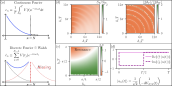
\includegraphics[scale=1]{../visual_elements/figs/alias_sqwave_res_polariton_full.pdf}
    \caption{
    (a) plots of the coefficients for the continuous Fourier transform, $c_n$, and discrete Fourier transform, $\tilde{c}_n$, in the case of a square wave. The difference arises due to the nature of the discrete time, which leads to the aliasing effect in the discrete Fourier coefficients. 
    (b) equivalent comparison between localization and error as in Fig.~5(b) from the main text but for a square wave drive. 
    (c) participation entropy for the spin-down component of a two-level system state for a kick drive which suffers from delocalization due to a Fourier polariton (spin-photon entanglement) near $h_z=\omega/2$. 
    (d) example of a Walsh polariton where the two spin components differ by a factor of a Walsh function. Not shown real and imaginary parts vanish.
    }
    \label{fig:Endmatter}
\end{figure*}

In the continuous Fourier case, we implement a hard cutoff at $n=N$. However, in the case of the discrete Fourier (and Walsh basis), the entire spectrum is mapped to within the cutoff. This is shown in Fig.~\ref{fig:Endmatter} by the red aliasing copy which adds together with infinitely many copies to give the (blue) discrete spectrum in the first zone. 

\section{Time Translation Generator}\label{sec:Time}

\subsection{Definition and Derivation}
The operator of interest is the derivative operator of the Schrödinger equation. Crucially, this operator is also the generator of time translations. When we work in a finite, non-analytic basis, such as the Walsh basis, the derivative and the generator of translations do not have the same spectrum for a finite truncation, so they must be distinguished from one another. This is seen partly due to the failure of the typical Taylor series argument, that establishes the correspondence between the two operators, which cannot be employed for the elements of the non-analytic Walsh basis.

To yield the correct results when we compare with other bases, we must explicitly use the generator of time translations. We construct the operator for discrete time translations of size $\Delta t$ and then scale appropriately to get an approximation to a continuum operator for arbitrary translations.

To understand time translations, we first need to define the vector space the operators act on. The Walsh basis and the discrete Fourier basis are defined using only a discrete set of times $t_j = j T/N$. Essentially, we take some function defined on the continuum, $f(t)$, and then map it onto a vector where the components represent the different times:
\begin{equation}
f(t) \mapsto
    \mathbf{f} = \begin{pmatrix}
f(t_0) \\
f(t_1) \\
f(t_2) \\
\vdots \\
f(t_{N-1})
\end{pmatrix}
\end{equation}



To generate time translations, we use a \textit{discrete time translation operator}. This is the cyclic left-shift matrix given by 
\begin{equation}
    \mathbf{T} = \begin{pmatrix}
0 & 1 & 0 & \cdots & 0 & 0 \\
0 & 0 & 1 & \cdots & 0 & 0 \\
0 & 0 & 0 & \cdots & 0 & 0 \\
\vdots & \vdots & \vdots & \ddots & \vdots & \vdots \\
0 & 0 & 0 & \cdots & 0 & 1 \\
1 & 0 & 0 & \cdots & 0 & 0
\end{pmatrix},
\label{eqn:translation}
\end{equation}
which performs the transformation $f(t_n) \mapsto f_T(t_n)=f(t_{n+1})=f(t_n+T/N)$. We employ periodic boundary conditions due to the periodic basis. Taking the matrix logarithm, we find the generator of time translations:
\begin{equation}
\label{eq:T_and_G}
    \mathbf{T} = \exp( \hat{G} T/N) 
    \quad\longrightarrow\quad \hat{G} = \frac{N}{T}\log(\mathbf{T}). 
\end{equation}
This operator $\hat{G}$ is a good approximation to the true generator of continuous time translations in the infinite Hilbert space since their truncated spectra are identical. Visualizing $\hat{G}$ as a matrix, it has the form shown in Fig.~\ref{fig:realspacederiv}. 

\begin{figure}[t!]
    \centering
    \includegraphics[width=\linewidth]{../visual_elements/figs/discrete_generator.pdf}
    \caption{A plot of the real and imaginary matrix elements of $\hat{G}$, cf.~Eq.~\eqref{eq:T_and_G}, when written in real space (i.e., not in Fourier space) for $N=64$. While the real part appears similar to the derivative, as expected, there is a broadening of non-zero values around the central diagonal due to the finite discretization.
    }
    \label{fig:realspacederiv}
\end{figure}

A guess for an antisymmetric derivative matrix could use finite differences like $\sim f(t_n) - f(t_{n-2})$, which $\hat{G}$ does have in addition to further contributions (See Fig.~\ref{fig:realspacederiv}). However, unlike the naive guess, the spectrum of $\hat{G}$ exactly matches that of the true derivative in the continuum at any finite truncation.

To convert the time translation operator into the space of the Walsh basis or into the discrete Fourier basis, we use their respective transformation matrices (Hadamard and cyclic exponentials). Combining the generator of time translations with the Hamiltonian in the Walsh basis to form $\bar{Q}=H-i\hat{G}$, we arrive at the matrix shown schematically in Fig.~\ref{fig:appendixQmatrix}. 

\begin{figure}
    \centering
    \includegraphics[scale=1]{../visual_elements/figs/H_extended_kick.pdf}
    \caption{Schematic of the quasienergy operator in the Fourier and Walsh bases for a periodic up-down kick drive. The matrix elements of the drive are shown in red, whereas the terms from the time-translation operator are shown in blue. (a) the quasienergy operator in the Fourier basis has a uniform all-to-all coupling via the kick drive elements. (b) in the Walsh basis, the time-translation operator is block diagonal.}
    \label{fig:appendixQmatrix}
\end{figure}

In Fig.~\ref{fig:appendixQmatrix}(b), we show the discrete time translation generator in blue in the Walsh basis. In contrast to the Fourier basis, it is block diagonal in natural ordering, but with relatively sparse blocks. The symmetry operation corresponding to the blocks acts on subsets of Walsh functions with the same smallest unit cell such that translations permute between these subsets.

The spectrum is identical to the truncated continuum operator which is just integer multiples of $\omega$. We find that all the odd multiples (i.e $\pm\omega, \pm 3\omega, \pm5\omega, \dots$) are associated with the large block in the lower right corner for the Walsh basis. For the diagonal blocks higher up, the spectrum of the block is odd integers multiplied by $2^b$ where $b$ labels the block number starting from zero in the bottom right.

\subsection{Representation in Walsh Basis}
As discussed in the main text, the rows of the Hadamard matrices are the Walsh basis functions. The translation operator by $T/4$ in the Walsh basis for $N=4$ is given by 

\begin{equation}
    \mathbf{T}_\text{Walsh}=\exp(\hat{G}T/4)=\begin{pmatrix}
        1& 0 & 0 & 0\\
        0 & -1 & 0 & 0 \\
        0 & 0 & 0 & -1 \\
        0 & 0& 1 & 0 \\
    \end{pmatrix}.
    \label{eqn:translationWalsh}
\end{equation}

This form makes sense since both $W_0$ and $W_1$ from Fig.~2(a) map to themselves (up to a minus sign) under translation by $T/4$, and $W_2$ and $W_3$ map to each other up to a minus sign. This is numerically calculated for larger $N$ by converting Eq.~\eqref{eqn:translation} into the Walsh basis using the Hadamard matrices: $ \frac{1}{N} \mathbb{H}_{N}\mathbf{T} \mathbb{H}_{N}=\mathbf{T}_\text{Walsh}$. 

Rewriting $T=2\pi/\omega$, and taking the matrix logarithm of Eq.~\eqref{eqn:translationWalsh}, we find
\begin{equation}
    \hat{G} = \frac{2\omega}{\pi}\begin{pmatrix}
        0& 0 & 0 & 0\\
        0 & i\pi & 0 & 0 \\
        0 & 0 & 0 & -\frac{\pi}{2} \\
        0 & 0& \frac{\pi}{2} & 0 \\
    \end{pmatrix}= \begin{pmatrix}
        0& 0 & 0 & 0\\
        0 & i2\omega & 0 & 0 \\
        0 & 0 & 0 & -\omega \\
        0 & 0& \omega & 0 \\
    \end{pmatrix}.
    \label{eqn:derivWalshN=4}
\end{equation}

As discussed earlier, this has the correct spectrum of multiples of $\omega$ for $i\partial_t \equiv i\hat{G}$ as we expect in the full continuum for Fourier. The block diagonal structure is also already evident, and it is also preserved for larger $N$.




\subsection{Symmetrization of Walsh Eigenvalues}

Due to the definition of the translation operator in the Walsh basis, the quasienergy spectrum is inherently asymmetric for the Walsh basis. We can see the asymmetry of the spectrum directly in the case of the resonances in Fig.~4(a) and explicitly in the construction from Eq.~\eqref{eqn:derivWalshN=4}.

The case $N=4$, (for $-i\partial_t\equiv -i\hat{G}$), yields eigenvalues $(-2\omega, -\omega, 0, \omega)$. In principle, we can symmetrize this spectrum by eliminating the lowest eigenvalue which can be performed for any $N$. For the drive elements, this means removing some rows and columns associated with $-2\omega$, thus removing $W_3$ from the basis. Under symmetrization, the translation generator of Eq.~\eqref{eqn:derivWalshN=4} becomes
\begin{equation}
\begin{pmatrix}
        0& 0 & 0 & 0\\
        0 & i2\omega & 0 & 0 \\
        0 & 0 & 0 & -\omega \\
        0 & 0& \omega & 0 \\
    \end{pmatrix} \rightarrow \begin{pmatrix}
        0 & 0 & 0\\
        0 & 0 & -\omega \\
         0& \omega & 0 \\
    \end{pmatrix},
\end{equation}
which now has a symmetric spectrum $(-i\omega, 0, i\omega).$

Alternatively, we have the freedom to also take $( -\omega, 0, \omega, 2\omega)$ since either $\pm 2\omega$ produce a minus sign from discrete translation. One could devise increasingly contrived symmetrization methods such as averaging out the effects of these two different cases to see if that produces better results. In fine-tuned problems, these techniques can be used to obtain more accurate solutions; however, they come at the cost of removing the completeness alongside the group structure and symmetry inherent in the Walsh basis. Hence, in this work, we have generally opted not to apply this procedure. 

\section{Truncation of Quasienergy Operator}\label{sec:Truncation}
The quasienergy phases, $\theta=\varepsilon T$, can be calculated from the eigenvalues of the quasienergy operator $\bar{Q}$. As discussed in the main text, this operator is infinite in extent, since we can couple states with arbitrarily many photons with an arbitrarily high-order process. The eigenvalues of the matrix can be numerically approximated by performing exact diagonalisation on a truncated version of the matrix.

In the case of the Fourier basis, we pick a finite number of basis elements for the space $\mathcal{L}_\odot$ by truncating to $\mathcal{L}^{(2M+1)}_\odot = \{e^{-iM\omega t}, \dots, e^{-i\omega t}, 1, e^{i\omega t}, \dots, e^{iM\omega t} \}$. This is described as ``truncating the frequency lattice" since we only take a finite number of ``sites" corresponding to different multiples of $\omega$. We then calculate the matrix elements of $\bar{Q}$ corresponding to this finite set of functions (using Eq.~2) and store them in an array (Fig.~\ref{fig:appendixQmatrix}) which we exactly diagonalize. The procedure is identical for the Walsh basis except we expand in the basis $\mathcal{L}^{(N)}_\odot = \{W_0(t), W_1(t), \dots, W_{N-1}(t)\}$.

\section{Square Drive Localization vs. Error}\label{sec:Square}
The basis of square functions, the Walsh basis, does not outpeform the Fourier for a square wave drive in the shape of $W_{N/2}(t)$. In Fig.~\ref{fig:Endmatter}(b), we compare the error to the localization as in Fig.~5(c) in the main text. For a square wave drive, the quasienergy error is at least an order of magnitude smaller for Fourier than Walsh. This surprising result follows from the response being approximately the integral of the drive at high frequency (Eq.~\eqref{eqn:vVleck}); a square wave drive has a triangle wave response, which requires fewer harmonics in the Fourier basis than the Walsh. 

The participation entropy correctly predicts the hierarchy of Walsh vs.~Fourier, and both error and entropy possess a similar ring structure (Fig.~\ref{fig:Endmatter}(b)); however, the maxima of the entropy rings are at odd multiples of $\pi$, whereas the maxima of the quasienergy rings are at even multiples of $\pi$. This discrepancy demonstrates the shortcomings of the localization measure; the Fourier spectrum for even multiples of $\pi$ consists of a single mode which results in a highly localized signature, suggesting the error is far better than it actually is. 

\section{Scaling of Errors with Number of Modes}\label{sec:Scaling}
We now discuss the scaling of the quasienergy errors with respect to various parameters in the two bases in the many-body case (Eq.~3) and single-particle case (Eq.~3 with $J=0$). We pick some illustrative values of $h_x, h_z$ such that we are firmly in the high-frequency regime. The two key parameters of interest for our systems are the driving frequency, $\omega$, and the number of elements we keep before truncation, $N$.

For the case of a square drive, we find that the quasienergy error in each case scales as 
\begin{equation}
    \Delta \theta_{\text{Fourier}} \sim N^{-3} \omega^{-3},\qquad
\Delta \theta_{\text{Walsh}} \sim N^{-2} \omega^{-3}.
\end{equation}
In general, the $\omega$ scaling of the error is universal for sufficiently weak drives since then the problem becomes equivalent to second-order perturbation theory about a diagonal derivative term with energy difference $\sim \omega$. For the square wave drive (Fig.~\ref{fig:errorscaling}(a)), we show that the Walsh fails to outperform the Fourier basis in this particular case, even with increasing $N$. This observation is in agreement with Fig.~\ref{fig:Endmatter}(b) and the associated single-particle localization theory that we explore in the main text. For the strongly driven regime of a kick drive, the scaling in $N$ is non-universal, and also does not appear to have a power law form in general, as shown in the lower row of Fig.~\ref{fig:errorscaling}, but we do see that the Walsh continues to outperform Fourier over a range of $N$. 
\begin{figure}
    \centering
    \includegraphics[width=\linewidth]{../visual_elements/figs/error_scaling.pdf}
    \caption{Scaling of the quasienergy phase error in the first Floquet Brillouin zone, $\Delta \theta$, with number of modes, $N$ for Walsh (green) and Fourier (orange). (a) shows the error for a single-particle, and (b) shows the error for the many-body Hamiltonian (Eq.~3) with $J=1$ and $L=3$. The top row shows results for a square wave drive where both show power law convergence with $N$. The parameters are $\omega=50$ with $h_z=1$ and $h_x=6$. The bottom row is the error for the up-down kick drive where the convergence of the solutions is not self-evident and Walsh outperforms Fourier by at least an order of magnitude. The parameters are $\omega=10$ with $h_z=5.5$ and $h_x=0.2$.
    }
    \label{fig:errorscaling}
\end{figure}


In the case of particularly strong kicking and low frequency in the many-body case, it is possible to have many resonances; these spectral features are a challenge to capture, and they act as an obstacle to convergence in both the Walsh and Fourier bases for a few states. We observe this lack of convergence for $\theta$ with increasing $N$ for the parameters of Fig.~4(a) in the main text; the corresponding scaling is shown in the right panel of Fig.~\ref{fig:nonconverge}. However, parts of the spectrum mostly unaffected by resonances can show order of magnitude smaller errors, but will not necessarily converge too. In contrast, the single-particle case converges for much stronger strong kicks (left panel of Fig.~\ref{fig:nonconverge}).

\begin{figure}
    \centering
    \includegraphics[width=\linewidth]{../visual_elements/figs/strong_kick_error_scaling.pdf}
    \caption{Convergence analysis for the same parameters in Fig.~4(a) for different kick strengths, $h_x$. While strong kicks ($h_x \sim \pi/2$) converge for the single-particle case (left panel), for many-body (right panel), even moderately strong kicks fail to converge. The large error is due to few states affected strongly by resonances as can be seen in Fig.~4(a).}
    \label{fig:nonconverge}
\end{figure}
\section{Expansion Coefficients of Walsh Basis for the Up-Down Kick Drive}\label{sec:Expansion}
The up-down kick drive consists of a positive delta pulse at $t=0$ and a negative pulse at $t=T/2$ (see Fig.~1(a) in the main text). There are two conventions one can use to discretize this function illustrated in Fig.~\ref{fig:appendixkick}; we can either symmetrically split the peak at $t=0$ into two ``half" delta functions (symmetric, as in (a)), or shift the delta peak by $\delta t=\epsilon>0$ to the right (non-symmetric, as in (b)). From a Floquet perspective, these correspond to shifting the Floquet gauge~\cite{Bukov2015}, $t_0$, which affects none of our results concerning quasienergies. 

In the main text, we use the symmetrized convention because it has fewer non-zero coefficients; only Walsh functions with opposite signs at $t=0$ and $t=T/2$ have non-zero overlap with the symmetrized up-down kick. These are easiest to study using sequency ordering \cite{Zhihua1983}, since this makes direct reference to the number of roots which dictates the signs at the points of interest. Walsh functions with an odd sequency start and end with an opposite sign. Doubling the sequency places the functions reflected end to end. Hence, only Walsh functions which have double an odd sequency, $m_\text{allowed} = 4m+2$ where $m\in \mathbb{N}$, are allowed. Thus, we find that $V_{\uparrow \downarrow,\text{s}}(t)= 2 \sum_{m=0}^\infty \mathcal{W}_{4m+2}(t)$. 

For the non-symmetrized convention, there are twice as many modes in the expansion: $V_{\uparrow \downarrow, \text{n}}(t)= 2\left( \sum_{m=0}^\infty \mathcal{W}_{4m+1}(t)+\mathcal{W}_{4m+2}(t) \right).$ 

\section{Strong Spin-Photon Hybridization (Walsh Polariton)}\label{sec:Strong}
While in the main text we only show the spin-up component, the spin-down component can be quite different in character. This is shown in Fig.~\ref{fig:Endmatter}(d).

We describe the strong hybridisation of spin and photon degrees of freedom as a polariton in the system. On resonance, generically in the limit of arbitrarily weak driving, we observe polariton states. These lead to significant errors for the Walsh basis, since the photon is associated with a factor $e^{im\omega t}$ which is strongly delocalized for the Walsh. This means that while these resonances lead to relative translations between spin component Fourier modes, leaving the localization unchanged, they drastically change the behavior of the localization between the spin degrees of freedom in the Walsh basis.

In the limit of strong driving, it is also possible to get Walsh polaritons as we observed for the kick with strength $\pi/2$; the two different spin components have a relative Walsh function time dependence between them. This could be observed in experimental platforms such as digital quantum simulators or NISQ devices. 


\section{Inverse-Frequency Expansion in the Walsh basis}\label{sec:Inverse-Frequency}

For a digital drive that takes constant values on certain intervals, we label the value of the Hamiltonian on time interval starting at $t_j$ by $H(t_{j})=H_{j}$. Thus, the unitary evolution operator in the case where we have $N=2^n$ intervals is given by
\begin{equation}
    U(T) = \prod^{\leftarrow}_{j} \exp\left( -\frac{iH_{j}T}{N}\right)\equiv \exp(-iH_{\text{eff}}T),
\end{equation}
where the product runs from earlier to later times, as indicated by the arrow. By using a generalized version of the Baker-Campbell-Hausdorff expansion (BCH) where we allow for arbitrary products, we can write an expansion for $H_\text{eff}$ in terms of $T$. For $N=2$, we recover the usual BCH expansion:
\begin{equation}
    H_{\text{eff}, N=2} = \frac{H_{0}+H_{1}}{2}- \frac{iT}{8}[H_{1},H_{0}]+\cdots\, .
\end{equation}


\begin{figure}[t!]
    \centering
    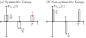
\includegraphics[width=\linewidth]{../visual_elements/figs/kick_gauge.pdf}
    \caption{(a) symmetric convention and (b) non-symmetric convention for discretizing the up-down periodic kick drive ($V_{\uparrow \downarrow}$).}
    \label{fig:appendixkick}
\end{figure}

For the case of general $N$, we compound the formula by splitting the time intervals for $H_0$ and $H_1$ as well. In the real space (time basis), the effective Hamiltonian can be expressed as 
\begin{equation}
    H_{\text{eff},N}=\bar{H}-\frac{iT}{2N^2} \sum_{i>j} [H_{i},H_{j}]+ \mathcal{O} \left( \frac{T^2}{N^3} \right).
\end{equation}
This is the most natural way to frame the problem in the Walsh basis since it is inherently defined only at discrete times. 

To convert this into the Walsh basis, we perform a Walsh-Hadamard transformation of the Hamiltonian. We define the new coefficients as 
\begin{equation}
    H_{j}=H(t_j)=\sum_{m=0}^{N-1}h_{m}  W_{mj},
\end{equation}
where the symmetric Hadamard matrix is defined by $W_{mj} \equiv W_m(t_j)$. If we substitute this form in, we get the expansion
\begin{equation}
    H_{\text{eff},N}= h_0 + iT\sum_{a>b} f_{ab}[h_a,h_b] +\cdots,
\end{equation}
where
\begin{equation}
    f_{ab} = -\frac{1}{N^2}\sum_{\alpha > \beta} W_{\alpha a} W_{\beta b}
    \label{eqn:deffab}
\end{equation}
defines the coefficients. We restrict the sum using a redundancy to $f_{ab} = -f_{ba}$~\footnote{The anti-symmetry follows from the fact that $f_{ab}+f_{ba}= \sum_{\alpha> \beta} W_{\alpha a}W_{\beta b}+ \sum_{\beta > \alpha}W_{\alpha a}W_{\beta b} = \sum_{\alpha,\beta} W_{\alpha a} W_{\beta b} \propto \delta_{a0}\delta_{b0}$ which is zero for all non-zero commutator terms.} which cancels the factor of $1/2$  in the series expansion. The factor of $1/N^2$ is included in Eq.~\eqref{eqn:deffab} to make $f_{ab}$ $N$-independent; this allows us to tabulate values for $f_{ab}$ that can be used for any number of basis functions. The matrix $f_{ab}$ has a number of non-zero elements that scales linearly with the basis size, much like in the Floquet-Magnus expansion \cite{BLANES2009}. 

We tabulate some non-zero values of the matrix according to their sequency labels (in contrast to the natural ordering used in the main text) since then these coefficients hold true for all $N$.

\begin{table}[ht]
    \centering
    \begin{tabular}{>{\centering\arraybackslash}p{2.5cm} >{\centering\arraybackslash}p{6.1cm}}
    \textbf{$f_{ab}$} & \textbf{$(a,b)$ (Sequency Labels)} \\
    \hline
    $2^{-2}$ & (1, 0) \\
    $2^{-3}$ & (3,0), (2, 1) \\
    $2^{-4}$ & (7, 0), (6, 1), (5, 2), (4,3) \\
    $2^{-5}$ & (15, 0), (14,1), (13, 2), (12, 3),\\ & (11, 4), (10, 5), (9, 6), (8,7) \\ 

    \end{tabular}
    \caption{Values of the first order term coefficient $f_{ab}$ in Eq.~\eqref{eqn:deffab} in the Walsh high-frequency expansion. All non-zero terms tabulated with magnitude greater than or equal to $2^{-5}$.}
    \label{table:fab}
\end{table}


We now apply this expansion to a few examples.
Consider a single spin $1/2$ driven by an up-down kick drive with 
\begin{equation}
    \hat{H}(t)= B_z \sigma^z+\Delta V_{\uparrow \downarrow,\text{n}}(t) \sigma^x.
\end{equation}
From the Baker-Campbell-Hausdorff expansion, we find that $H_\text{eff}=B_z \sigma^z+ B_z\Delta \sigma^y+\mathcal{O}(\Delta^2)$. The expansion is sensitive to the Floquet gauge in this case (see Sec.~\ref{sec:Expansion}), so using the non-symmetrized gauge with $f_{10}=1/4$ and coefficient $h_1=\frac{2}{T}\Delta \sigma^x$, we recover the same result. If we use the symmetrized gauge, the first order term vanishes such that $H_\text{eff}'=B_z \sigma^z +\mathcal{O}(\Delta^2)$ which is equivalent to a Schrieffer-Wolff transformation on $H_\text{eff}$ \cite{Bravyi2011}.

To demonstrate the utility of the Walsh expansion, we study a two-tone driving of the form
\begin{equation}
    \hat{H}(t)=B_z \sigma^z+ W_2(t) B_x \sigma^x+W_{13}(t) B_y \sigma^y,
\end{equation}
where $W_a(t)$ is the Walsh function labelled with sequency. Due to the frequent flipping of $W_{13}(t)$ (Fig.~\ref{fig:serieserror}(a)), a BCH-type expansion involves several steps. However, from a single commutator in the Walsh expansion, we find the relevant first order correction to be
\begin{equation}
    H_{\text{eff}}^{(1)}=\frac{T}{16}B_x B_y\sigma^z.
    \label{eqn:complicateddrive}
\end{equation}

We validate this result by numerically calculating the full evolution, $H_F$, and studying the scaling with frequency $\omega=2\pi/T$ after subtracting off terms calculated from the series. Removing the zero order contribution, $H_\text{eff}^{(0)}\sim\mathcal{O}(\omega^0)$ (shown in blue in Fig.~\ref{fig:serieserror}(a)), means the dominant omega scaling is $\omega^{-1}$. Also removing the correct first order term, $H_\text{eff}^{(1)} \sim \mathcal{O}(\omega^{-1})$ (shown in orange in Fig.~\ref{fig:serieserror}(a)), gives a dominant scaling of $\omega^{-2}$. On a log-log plot, the power law dependence of the remaining dominant contribution in the series is a linear trend, and the slopes are in agreement with the predicted $\omega$ scaling demonstrates that Eq.~\eqref{eqn:complicateddrive} is correct.

While the Walsh basis effectively condenses the $N^2$ commutators in the BCH expansion to $N$ terms or less, there is a trade-off in the complexity of each individual commutator term. Here, symbolic approaches may be helpful in combination with the techniques developed in our work \cite{SandovalSantana2019}.

\begin{figure}[ht!]
    \centering
    \includegraphics[width=\linewidth]{../visual_elements/figs/walsh_series.pdf}
    \caption{(a) Walsh function $W_{13}(t)$ with a sequency of 13. \\(b) difference between Walsh series and true Floquet Hamiltonian for $\hat{H}(t)=B_z \sigma^z+ W_2(t) B_x \sigma^x+W_{13}(t) B_y \sigma^y$. The eigenvalues, $\Delta \varepsilon$ of the remainder $H_F-H^{(0+1)}_\text{eff} \equiv H_F-H^{(0)}_\text{eff}-H^{(1)}_\text{eff}\sim \omega^{-2}$ demonstrating that the first order correction successfully canceled contributions $\mathcal{O}(\omega^{-1})$.
    }
    \label{fig:serieserror}
\end{figure}

\pagebreak


% ---- References for the Supplemental (labels appear as [S1], [S2], …)
\bibliography{bibliography}

\end{document}
